\chapter{Theoretische Grundlagen}
\label{chap:theoretische_grundlagen} Dieses Kapitel führt in die theoretischen Grundlagen
ein, die in dieser Arbeit benötigt werden. Den ersten Teil bilden die domänenspezifischen
Grundlagen \ref{sec:domänenspezifisch}, welche genauer darauf eingehen, welchen Inhalt
die zu bearbeitenden Bilder bieten und wie dieser zu verstehen ist. Abschnitt
\ref{sec:technologisch} geht hierbei auf verschiedenen Technologien ein, die eine
wichtige Rolle spielen. Der Abschnitt \ref{sec:verwwandte_arbeit} geht auf die
Arbeit von \citet{hoffmann2020} ein und legte damit den Grundstein dieser Arbeit.
Die Abschnitte \ref{sec:3d_slicer} und \ref{sec:architektonisch} führen in
Softwareentwicklungsthemen ein, die zum Erstellen einer \textit{3D Slicer
Extention} wichtig sind.
% ---------------------------------------------------------------------------------------

\section{Domänenspezifisch}
\label{sec:domänenspezifisch} Wie bereits aus dem Kapitel \ref{chap:einleitung}
Einleitung klar wurde, handelt es sich bei den Micro-CT Bilder um Zahnbilder,
die aufgrund von Zahnkaries entfernt wurden. Um zu verstehen, wie eine CT-Aufnahme
eines Zahns aufgeteilt werden soll, ist es hilfreich zu verstehen, wie ein Zahn
aufgebaut ist.

\begin{minipage}{0.40\textwidth}
	Die Abbildung \ref{fig:aufbau_eines_zahnes} zeigt den groben Aufbau eines Zahnes
	nach \citet[Seite 17]{lehmann2012Zahnheilkunde}. Zu sehen ist, dass das Denit oder
	auch Zahnbein genannt, den Großteil eines Zahnes einnimmt. Im Bereich der Zahnkrone
	wird das Dentin von Zahnschmelz überzogen. Der Zahnschmelz ragt in die
	Mundhöhle und ist nach \cite[Seite 41]{lehmann2012Zahnheilkunde} das härteste
	Material im menschlichen Körper. In der Mitte des Zahnes befindet sich Weichgewebe,
	welches als Pulpa bezeichnet wird vgl. \citep[Seite ]{lehmann2012Zahnheilkunde}.
\end{minipage}
\hfill
\begin{minipage}{0.50\textwidth}
	\centering
	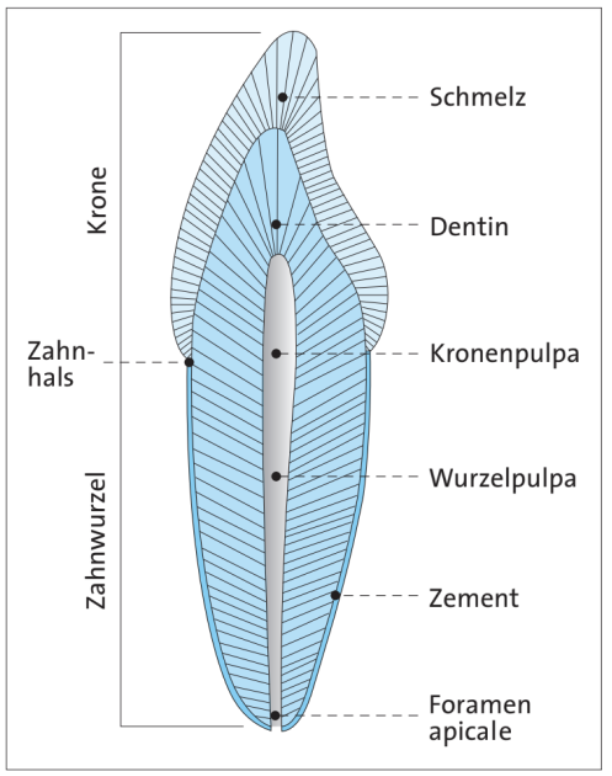
\includegraphics[scale=0.50]{img/aufbau_eines_zahns.jpg}
	\captionof{figure}{Aufbau eines Zahnes nach \citet{lehmann2012Zahnheilkunde}} \label{fig:aufbau_eines_zahnes}
\end{minipage}

Für die Bearbeitung von Micro-CT Aufnahmen sind die Bereich Schmelz Dentin und Pulpa
von besonderer Bedeutung. Betrachtet man eine CT wie es zu Beginn in der
Abbildung \ref{fig:ct_aufnahme_eines_zahns} gezeigt wurde, so bilden diese 3 Gewebearten
die unterschiedlichen Grauwerte in einem CT-Bild. \\ \textbf{Pulpa:} Die Pulpa unterscheidet
sich hierbei nur wenig vom Hintergrund, da sie als einzige der drei Hauptteile
eines Zahnes ein Weichgewebe ist und bei einer Röntgenaufnahme nicht absorbiert.
Geht man weiter von innen nach außen, so ist der nächste Zahnteil auf einem CT
das Zahnbein. \\ \textbf{Dentin:} Das Dentin ist laut \citet[Seite 41]{lehmann2012Zahnheilkunde}
eine Hartsubstanz, die dem Kieferknochen sehr nah steht. So kommt es, dass dieser
Teil schon deutlich besser auf einem CT zu erkennen ist. Den äußersten Teil in
der Mundhöhle bildet das Zahnschmelz. \\ \textbf{Schmelz:} Der Schmelz ist wie
bereits erwähnt, der härteste Teil im menschlichen Körper und aus diesem Grund auch
am hellsten auf dem CT zu erkennen. Die folgende Abbildung
\ref{fig:pulpa_dentin_schmelz} sollen durch Gegenüberstellung den Zusammenhang
zwischen einem CT-Bild und einer Zahnzeichnung verdeutlichen.

\begin{figure}[h]
	\centering
	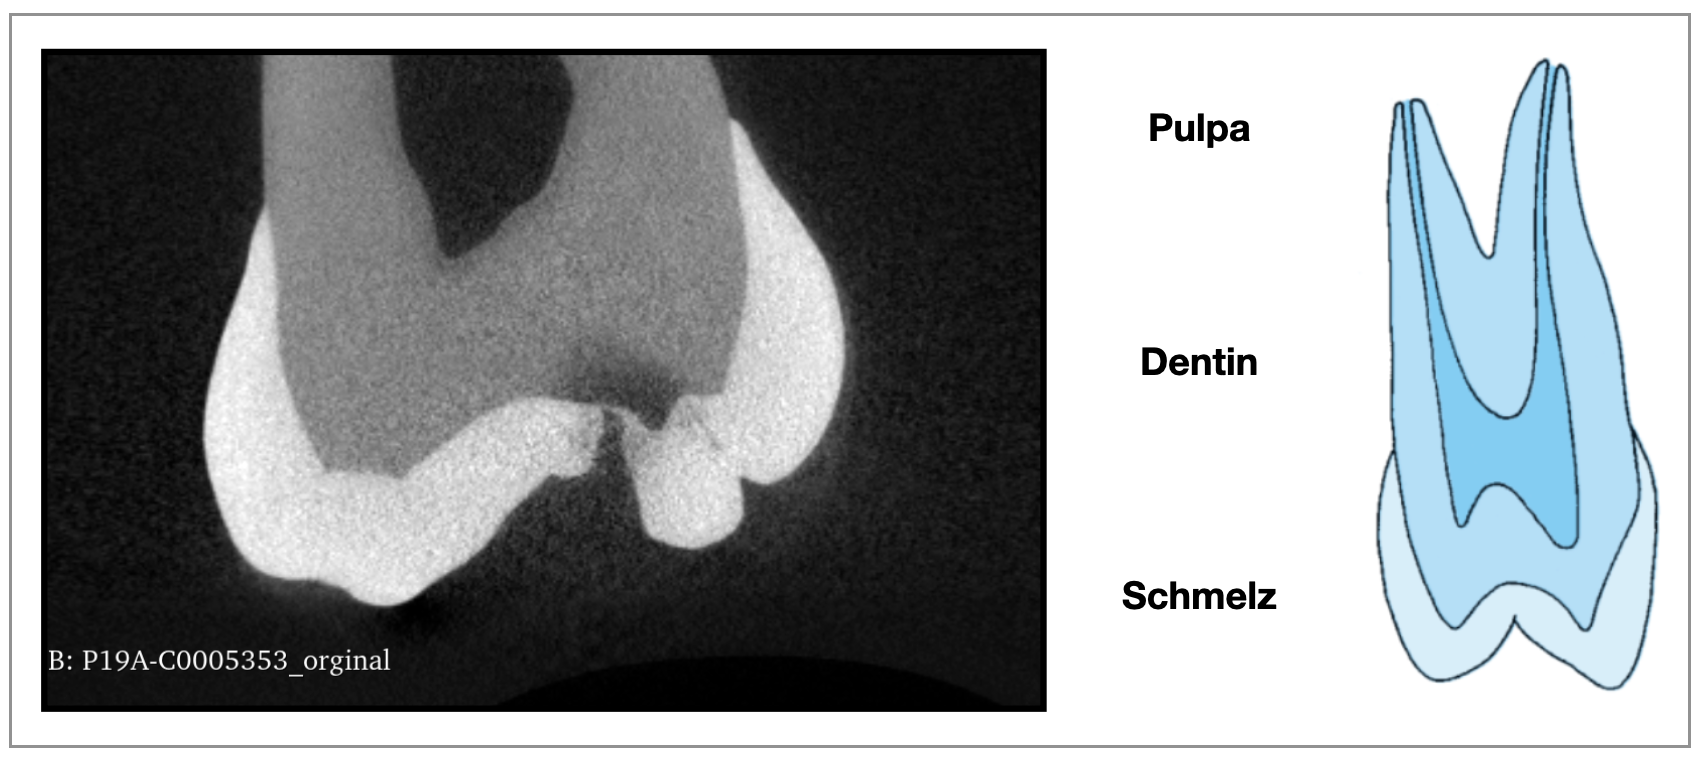
\includegraphics[width=0.9\textwidth]{
		img/Bildschirmfoto 2024-11-22 um 15.13.24.jpg
	}
	\caption{Darstellung von Pulpa, Dentin und Schmelz auf einer CT-Aufnahme (link)
	und einer Zeichnung (rechts) nach \citet[Seite 29]{lehmann2012Zahnheilkunde}. }
	\label{fig:pulpa_dentin_schmelz}
\end{figure}

Mit diesem Domänenwissen kann ein Schritt weiter gegangen werden, sodass der
Fokus nun auf die CT-Bilder gesetzt wird. Das Kapitel \ref{sec:technologisch} Technologien
führt die Technologie der Computertomografie tiefer ein. Mit diesem
Domänenwissen kann ein Schritt weiter gegangen werden, sodass der Fokus nun auf die
CT-Bilder gesetzt wird. Das Kapitel \ref{sec:technologisch} Technologien führt
die Technologie der Computertomografie tiefer ein.
% ---------------------------------------------------------------------------------------

\section{Technologisch}
\label{sec:technologisch} Dieser Abschnitt erläutert federführend die
Technologie der Micro-CT Bilder und deren weitere Bearbeitung. Hierbei soll mit der
Computertomografie selbst begonnen werden. Für die Einführung in die Bearbeitung
der Micro-CT Bilder bietet das Pipeline-Modell von \citet[Seite 50]{handels2000}
eine gute Richtlinie. Er beschreibt mit dieser Visualisierungs-Pipeline Schritte,
die bei der Bearbeitung und dreidimensionalen Darstellung von CT-Aufnahmen
notwendig sind (vgl. \citep[Seite 50]{handels2000}).
% ---------------------------------------------------------------------------------------

\subsection{Computertomografie}
\label{subsec:computertomografie} Die Erfindung der Computertomografie (CT) war ein
Quantensprung in der Geschichte der Medizin. Sie ist aus heutigen Diagnosen
nicht mehr wegzudenken. Ein Micro-CT Bild ist laut \citet[Abstract]{baird2017} ein
Menge hochauflösender Bilder, die wie ein Stapel zusammengelegt werden. Der Aspekt
Micro deutet dabei darauf hin, dass es eine miniaturisierte Ausführung eines
üblichen Kegelstrahl-CTs ist so \citet[Seite 340]{buzug2011}. Eine andere Definition
erläutert \citet{lehmann2013bildverarbeitung}. Er beschreibt die Computertomografie
als Projektionen einzelner Ebenen im Untersuchungsobjekt. Die Technologie, mit der
diese Bilderstapel aufgenommen werden, ist unter der Röntgentechnik oder auch X-Ray
bekannt. Die Röntgenstrahlung ist eine Form der elektromagnetischen Strahlung,
ähnlich wie da sichtbare Licht so das \citet{nib2024}. Anders als das Licht
haben die Röntgenstrahlen eine viel höhere Energie. Das führt dazu, dass man mit
dieser elektromagnetischen Strahlung viele Objekte durchdringen kann. So auch Gewebeteile
eines Zahnes vgl. \citep{nib2024}. Die Abbildung \ref{fig:spectrum} zeigt diese
elektromagnetische Spektrum.

\begin{figure}[h]
	\centering
	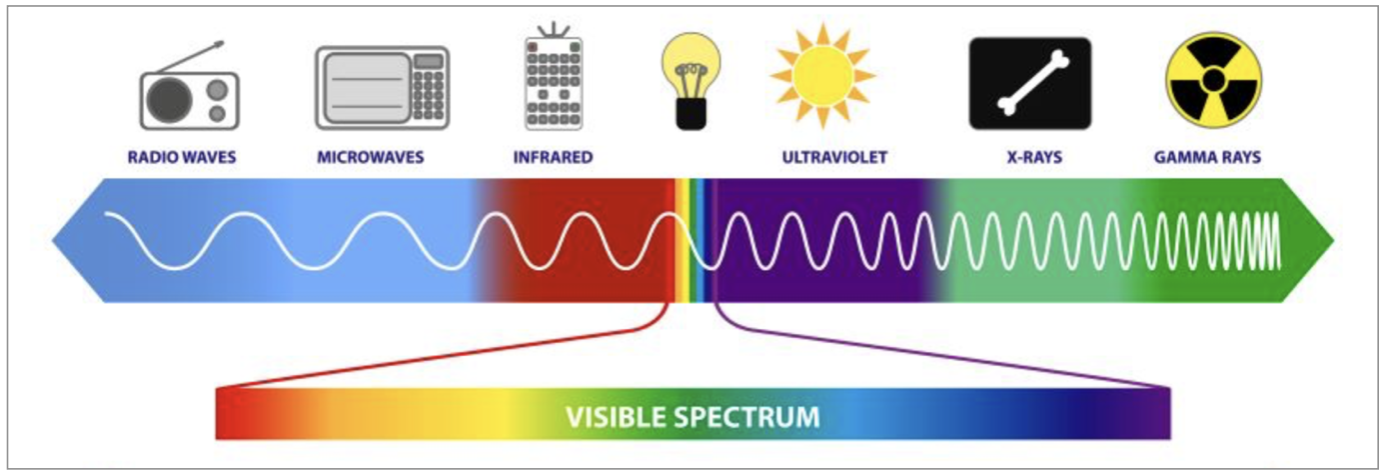
\includegraphics[width=0.9\textwidth]{img/spectrum.jpg}
	\caption{Einordnung der Röntgenstrahlung nach dem \citet{nib2024}}
	\label{fig:spectrum}
\end{figure}

Durchdringt ein solcher Röntgenstrahl ein Untersuchungsobjekt, werden die
Details aufgrund der Wechselwirkung mit Materie auf einer CT-Probe sichtbar. Die
bekannteste Wechselwirkung ist die Absorption. Mit der Steigerung der Atomzahl
in einem Material nimmt auch die Absorption eines Materials zu, sodass es leicht
ist verschiedenen Materialien in einer CT-Aufnahme zu unterscheiden \citep{nib2024}.

Für eine Micro-CT Aufnahme bedarf es spezieller Technik. Es gibt unterschiedliche
Firmen, welche die unterschiedlichsten Modelle anbieten. Im Falle der Zahnklinik
an der LMU in München handelt es sich um ein Micro-CT 40 der Firma \citet{scanco2024}.
Dieses Gerät erstellt Aufnahmen mittels Röntgenstrahlung und generiert mithilfe der
Computertomografie ein dreidimensionales Bild, welches im Format \texttt{.ISQ} abgelegt
wird. Wie das Nächste Kapitel beschreiben wird ist der Speicherumfang den solch
ein Bild benötigt, deutlich zu groß. Es bedarf einer Technik, mit der die Aufnahmen
auf eine handhabbare Größe schrumpfen.
% ---------------------------------------------------------------------------------------

\subsection{Datensätze}
\label{subsec:datensätze} Die rohen Datensätze, welche direkt aus dem Micro-CT
Gerät kommen, haben nach \citet{scanco2024} das Format \texttt{.ISQ}. Dieses
Format fällt speziell auf die Geräte der Firma SCANCO zurück. Wie das vorherige Kapitel
\ref{subsec:computertomografie} bereits eingeführt hat, ist dieser Dateityp für
eine weitere Bearbeitung nicht geeignet. Unter anderem wegen ihrer Größe. \citet{RoeschKunzelmann2018}
haben hierfür ein Paket entwickelt. Dieses konvertiert ein \texttt{.ISQ} Format in
ein \texttt{.mhd} Format. Bei einer \texttt{.mhd} Datei handelt es sich um ein
Metafile, dass auf die eigentliche Datei verweist. Folgender Ausschnitt zeigt
die Verwendung des Pakets.

\texttt{python3 isq\_to\_mhd.py <quelle> <ziel>}

Diese Meta-Datei kann genutzt werden, um interessante Informationen über das Bild
zu erlangen. Wird dieses Kommando ausgeführt, so erstellt das Skript \texttt{isq\_to\_mhd}
ein Metafile, das detailliert Daten über die Datei enthält. Ein Ausschnitt
dieses Metafiles liefer das Listing \ref{lst:inhalt_mhd_datei}

\begin{lstlisting}[
	caption={Ausschnitt des Inhaltes einer MHD-Datei},
	label={lst:inhalt_mhd_datei}]
ObjectType = Image
NDims = 3
CenterOfRotation = 0 0 0
ElementSpacing = 0.02 0.02 0.02
DimSize = 1024 1024 517
ElementType = MET_SHORT
ElementDataFile = P01A-C0005278.ISQ
\end{lstlisting}

In der Datei sind Informationen über die Ausprägung, Art und Größe der Datei zu finden.
Besonders interessant sind die Punkte \texttt{DimSize und ElementType}. Über
diese Parameter lässt sich die Größe eines Bildes berechnen. \citet[Seite 10-11]{burger2009}
erklärt, das ein Bild in Zellen aufgeteilt ist, welche Informationen enthalten.
Diese Zellen sind im zweidimensionalen Raum als Pixel bekannt. Betrachtet man jedoch
ein, wie im Falle der Zahnklinik an der LMU dreidimensionales Bild, so spricht man
nicht mehr von einem Pixeln, sondern von einem Voxel. Ein Voxel ist demnach das dreidimensionale
Äquivalent zu einem Pixel. \citet[Seite 10-11]{burger2009} beschreibt weiter das
jeder diese Zellen ein binäres Wort der Länge $2^{k}$ ist. Die Basis 2 ergibt sich
durch das binäre Wort, wo hingegen für $k$ gilt: $k \in \mathbb{N}$. Um für den
konkreten Fall aus Listing \ref{lst:inhalt_mhd_datei} das entsprechenden $k$ zu
ermitteln, muss der \texttt{ElementType} näher betrachtet werden. \texttt{MET\_SHORT}
steht hierbei für Signed short, was eine Größe von 16 Bit entspricht. Damit
ergibt sich für die Länge $k$ ein Wert von 4. So können nach \citet[Seite 10-11]{burger2009}
folgende Gleichungen festgehalten werden.

\begin{align}
	\label{equ:größe_bestimmen}1024 \cdot 1024 \cdot 517    & = 542,113,792 \, \text{Voxel}\notag  \\
	542,113,792 \, \text{Voxel}\cdot 2 \, \text{Byte/Voxel} & = 1,084,227,584 \, \text{Byte}\notag \\
	1,084,227,584 / 1,000,000,000                           & = 1.0842 \, \text{GB}
\end{align}

Die erste Gleichung bestimmt die Gesamtzahl aller Voxel in einem Bild. Gleichung
2 ermittelt die Größe des Bildes in der Einheit Byte. Die letzte Zeile nimmt eine
Umrechnung von Byte nach Gigabyte (GB) vor.

Durch die Gleichungen in \ref{equ:größe_bestimmen} wird klar, das eine CT-Aufnahme
des Typs \texttt{.ISQ} direkt nach seiner Aufnahme über einen GB groß ist. Laut
\citet{poliklinikLMU} ist dies ein zu großes Format. Es stellt sich also die
spannende Frage, wie solch eine Datei komprimiert werden kann, ohne das es
Verluste in der Qualität gibt. Dr. Elisa Walter hat hierfür eine Lösunge
entwickelt. QUELLE Betrachtet man den \texttt{ElementType} genauer, so fällt auf,
das es noch weiter Typen gibt, die durch eine geringerer Länge $k$ deutlich weniger
Speicher benötigen. Durch Anwendung simpler Statistik lässt sich herrauslesen, das
die $2^{4}$ Byte je Element nicht ausgenutzt werden. Als Werkzeug für die
Betrachtung einer solchen Statistik kann das Histogramm eines Bildes genuztzt
werden. Diese zeigt Grafisch die unterschiedlichen Grauwerte (X-Achse) zu ihren Häufigkeiten
im Bild (Y-Achse) Werden einige der Argumente nicht verwenden, so kann der
\texttt{ElementTyp} verkleinert werden

\subsection{Filter}

\subsection{Segmentierung}

\section{Verwandte Arbeit}
\label{sec:verwwandte_arbeit}

\section{3D Slicer}
\label{sec:3d_slicer}

\subsection{Extention Manager}

\subsection{Python Umgebung}

\subsection{MRML Datenstruktur}

\subsection{Qt-Designer}

\section{Architektonisch}
\label{sec:architektonisch}